\chapter{Distributed Databases}
For several decades, centralized database management systems running on a single database server have been predominant, for these four main reasons:
\begin{itemize}
    \item \textit{Complexity} of a single-server system was lower and administration easier
    \item \textit{Evaluate short queries} and \textit{infrequent data modification}
    \item \textit{Slow network} so sending large amount of data was too costly
    \item \textit{Parallelization} required rewriting a query into subqueries and recombining the results, overhead diminished the positive effects of a parallel execution of subqueries
\end{itemize}
Whenever there were more demanding requirements:
\begin{itemize}
    \item \textbf{Scaling up} or \textbf{Vertical scaling} equip the single database server with higher hardware capacity
    \begin{itemize}
        \item Amount of data and queries a single database server can handle is limited
        \item A single server is always a single point of failure
    \end{itemize}
    \item \textbf{Scaling out} or \textbf{Horizontal scaling} connecting several cheaper servers in a network
    \begin{itemize}
        \item The only option to improve the throughput and latency of a database system
        \item Disadvantage of cost of coordination and synchronization of the database servers
        \item However this last one pays off for large scale systems or global enterprises with several data centers
    \end{itemize}
\end{itemize}

\section{Scaling Horizontally}
\begin{itemize}
    \item The ability of a database system to \textit{flexibly scale out by distributing data in a server network} is called \textbf{horizontal scalability}
    \item Servers can work independently
    \item Also called \textbf{shared-nothing architecture}
    \item The most common use case today is a distributed database on a shared-nothing architecture
    \begin{itemize}
        \item A distributed database management system (DDBMS) that runs on a network of independent servers
        \item The servers need not be large
        \item They consist of cheaper commodity hardware so that each server can easily be replaced by a new one
    \end{itemize}
\end{itemize}
DBMS are benefical also when aiming for improved availability and reliability in smaller scaled systems:
\begin{itemize}
    \item \textbf{Load balancing:} user queries and other processes should be assigned to the servers in the network such that all servers have approximately the same load
    \item \textbf{Flexible scalability:} servers may flexibly leave and join the network at any time
    \item \textbf{Heterogeneous nodes:} servers may flexibly leave and join the network at any time
    \item \textbf{Symmetric configuration:} every node is configured identically to the others;
    \item \textbf{Decentralized control:} peer-to-peer algorithms for data management improve failure tolerance of a DDBMS
\end{itemize}

\section{Distribution Transparency}
For a user it must basically be transparent how the DBMS internally handles data storage and query processing in a distributed manner.
\begin{itemize}
    \item \textbf{Access transparency:} uniform query and management interface to users independent of the structure of the network
    \item \textbf{Location transparency:} the distribution of data in the database system is hidden from the user
    \item \textbf{Replication transparency:} if several copies of a data item are stored on different servers the user should not be aware of this
    \item \textbf{Fragmentation transparency:} if a large data set has to be split into several data items and the distributed database system does this splitting internally and the user can query the database as if it contained the entire unfragmented data set
    \item \textbf{Migration transparency:} if data items have to be moved from one server to another, this should not affect how a user accesses the data
    \item \textbf{Concurrency transparency:} when multiple users access the database system, their operation must not interfere or lead to incorrect data in the database system
    \item \textbf{Failure transparency:} as a distributed database system is more complex than a centralized one
\end{itemize}

\section{Failures in Distributed Systems}
\begin{itemize}
    \item \textbf{Server failure:} a DBS may fail to process messages due to notwork component crash or a self crash
    \begin{figure}[!h]
        \centering
        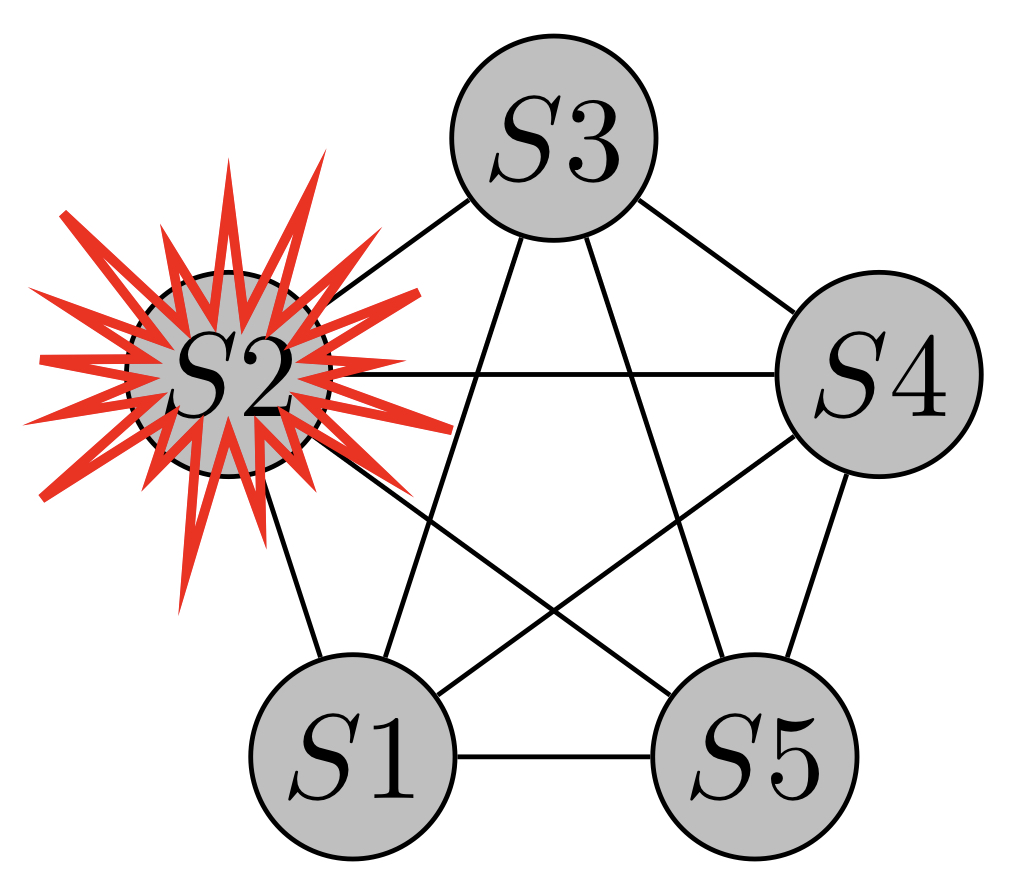
\includegraphics[width=0.2\linewidth]{images/AdvancedDataManagment/distributed_databases/server_failure.jpeg}
    \end{figure}
    
    \item \textbf{Message failures:} message through the network links may be delayed or lost during times of high congestion
    \item \textbf{Link failure:} a communication link between two servers may be unable to transmit messages. Note that a \textit{link failure} \textbf{can cause} a \textit{message failure}
    \begin{figure}[!h]
        \centering
        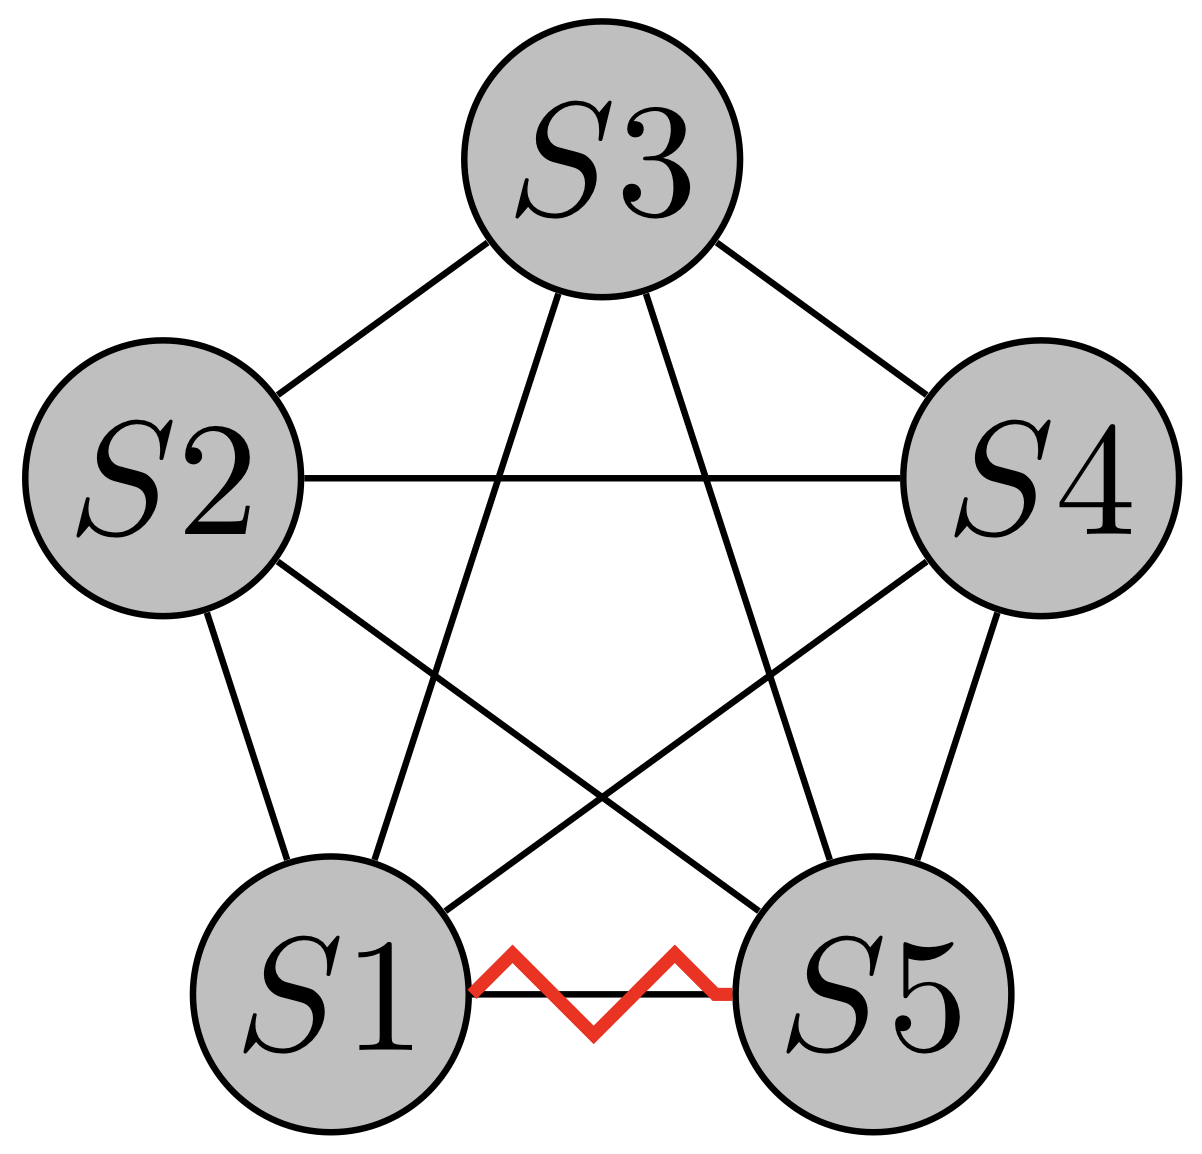
\includegraphics[width=0.2\linewidth]{images/AdvancedDataManagment/distributed_databases/link_failure.jpeg}
    \end{figure}
    \item \textbf{Network partition:} when the network is splitted into two or more subnetworks that are unable to communicate
    \begin{figure}[!h]
        \centering
        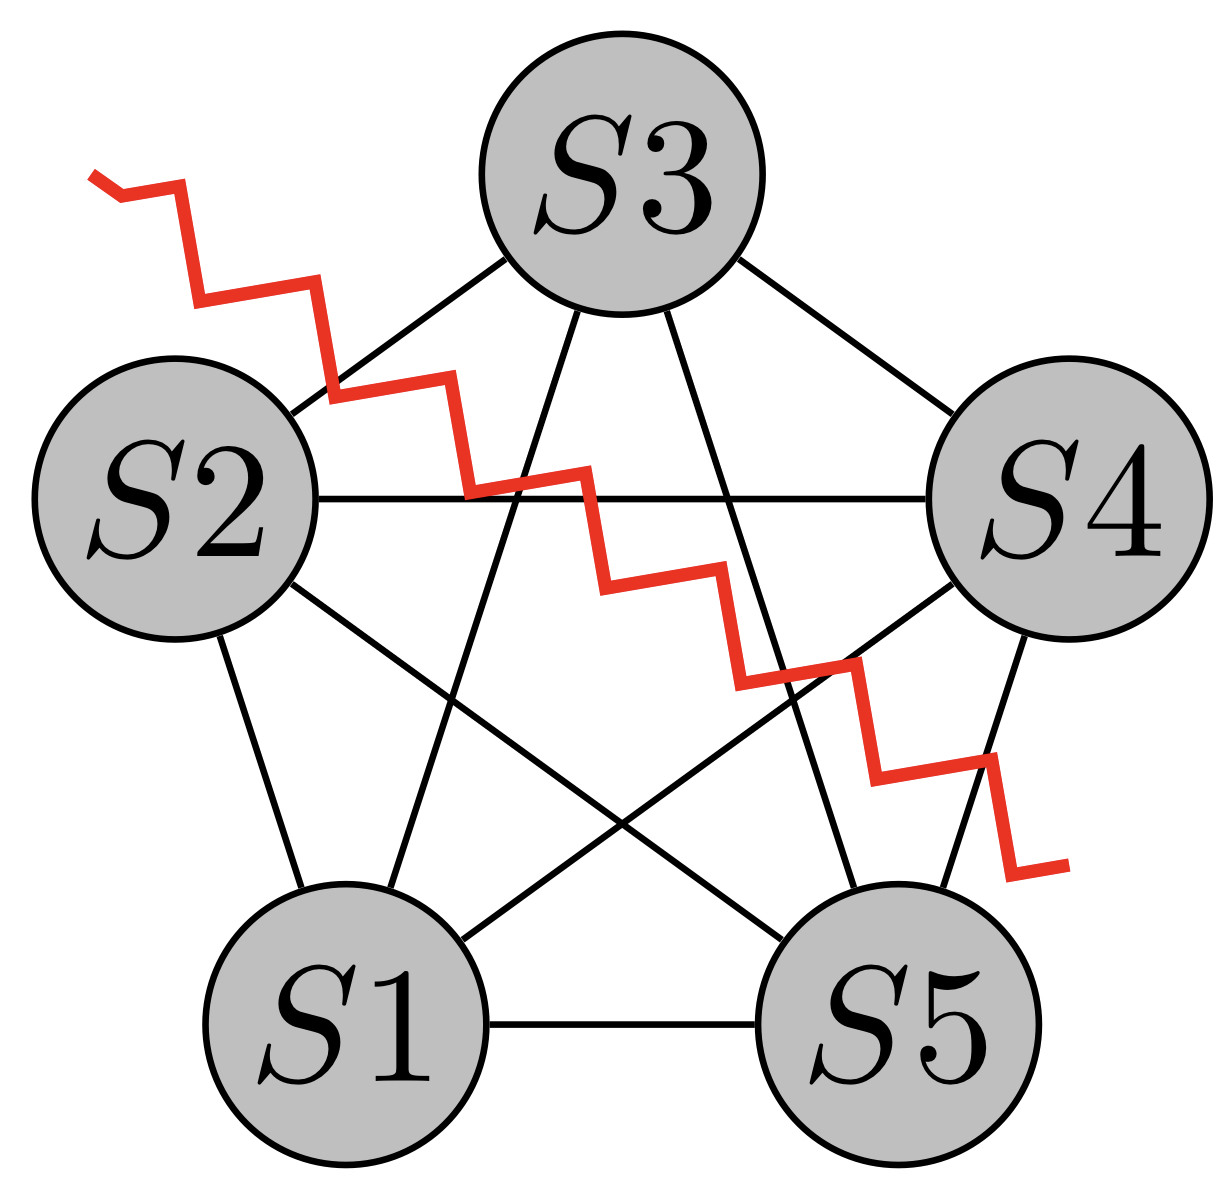
\includegraphics[width=0.2\linewidth]{images/AdvancedDataManagment/distributed_databases/network_partition.jpeg}
    \end{figure}
\end{itemize}

\textbf{Node Failure} can be categorized into:
\begin{itemize}
    \item \textbf{Crash failures:} is a permanent failure of a server and corresponds to aborting a communication protocol. Once the server crashed, it will never resume operation
    \item \textbf{Omission failures:} an omission failure corresponds to not taking some action
    \item \textbf{Commission failures:} corresponds to taking an action that is not correct according to  a communication protocol
\end{itemize}
Moreover we note that:
\begin{itemize}
    \item Crash failures are a special case of omission failures.
    \item The union of omission and commission failures is called \textbf{Byzantine failures}
    \item The term \textbf{non-Byzantine failures} usually refers to omission failures but in addition explicitly also covers duplication and reordering of messages
\end{itemize}

Distributed DBMSs have to provide a high level of \textbf{fault tolerance}, indeed, a distributed system may in general be design based on a certain \textbf{failure model} which describes the set of failures that the system can tolerate.
\begin{itemize}
    \item \textbf{Fail-stop model:} all server failures are crash failures that permanently render the server unavailable 
    \item \textbf{Fail-recover model:} a server may halt but it may later resume execution. The resumption could be:
    \begin{itemize}
        \item In the state before it was halted
        \item From scratch
    \end{itemize}
\end{itemize}

\section{Epidemic Protocols and Gossip Communication}
Due to the many properties  the propagation of information in the network is difficult to manage. In the \textit{simplest scenario} 
\begin{itemize}
    \item Whenever new information is received by one server, the server sends a notification to all the other servers he know
    \item But the initiating server might not be aware of all servers currently in the network
    \item Some of his messages might be lost due to network failures
\end{itemize}
\begin{tcolorbox}
An alternative is when the DBS can be seen as participants in a \textit{peer-to-peer network} where there is \textit{no central coordinator}. \textbf{Epidemic protocols} are a category of peer-to-peer algorithms, where information is spread like an infection all over the network
\end{tcolorbox}
An other application is \textbf{membership} of peers n the network:
\begin{itemize}
    \item Each server has to maintain a list of names
    \item This list can be kept up-to-date by an epidemic algorithm
    \item Servers exchange their membership lists in a peer-to-peer fashion so that the information which servers are part of the network slowly spreads over the entire network
\end{itemize}
With an epidemic algorithm, servers in the network pass on a message \textbf{like an infection}. A \textbf{message} notification that some new server has joined the network, so the servers that receive this message update their membership list.
We have three types of nodes:
\begin{itemize}
    \item \textbf{Infected nodes:} are servers that have received a new message that they want to pass on to others
    \item \textbf{Susceptible nodes:} are nodes that so far have not received the new message
    \item \textbf{Removed nodes:} are nodes that already have received the message but are no longer willing to pass it
\end{itemize}

There are three different communication modes that can be applied in epidemic algorithms:
\begin{itemize}
    \item \textbf{push-only:} an infected server contacts another server and passes on all the new messages it has received. Infected server \(\rightarrow\) susceptible server
    \item \textbf{pull-only:} a susceptible server contacts another server and asks for new messages. Susceptible server \(\rightarrow\) infected server
    \item \textbf{push-pull:} one server contacts another server and both
exchange their new messages. Both servers have the same state
\end{itemize}

A synonym for epidemic message exchange is \textbf{gossiping:} the term expresses that messages spread in a server network like rumors in human communication.

Two variants of epidemic algorithms for database updates are:
\begin{itemize}
    \item \textbf{Anti-entropy} is a periodic task that is scheduled for a fixed time span, for example every minute. It is called also \textit{simple epidemic} since any server is either susceptible or infective and the infection process \textit{does not degrade} over time or due to some probabilistic decision.
    \item \textbf{Rumor spreading} is an infection that can be triggered by the \textit{arrival of a new message} or it can be run periodically. Here the infection have several rounds, in each one a server chooses a set of communication partners (called \textit{fanout}). It is a \textit{complex epidemic} because infection of other servers is a dynamic process: amount of server decreases every round.
\end{itemize}
This decrease of infections can be varied as follows:
\begin{itemize}
        \item \textit{Probabilistic:} after each exchange with another server, the server stops being infective with a certain probability
        \item \textit{Counter-based:} After a certain number k of exchanges, the server stops being infective. Therer are two cases:
        \begin{itemize}
            \item \textit{Infect-and-die} the number k is equal to the fan-out
            \item \textit{Infect-forever} the number k is infinite and the server never stops
        \end{itemize}
        \item \textit{Blind:} the server becomes removed without taking the feedback of communication partners is into account
        \item \textit{Feedback-based:} the server becomes removed if it notices that the communication partners already have received the new message
    \end{itemize}
    
\subsection{Hash Trees}
A major issue with epidemic protocols is how two servers can identify those messages in which they differ. For example a complete comparison of all messages is not feasible as this would slow down the epidemic process tremendously.

A simple improvement is to use a \textbf{list of hash values}
\begin{itemize}
    \item Comparison of hash values is faster
    \item The downside, the hash values have to be computed and still the list of hash values has to be compared sequentially
\end{itemize}
A step further could be take using a \textbf{hash tree}:
\begin{itemize}
    \item It starts with a hash of each message in a leave node, and then iteratively concatenates hashes
    \item For \textit{inner node}, closer a hash value is to the root, the more leave it covers
    \item The last hash value at the root of the tree is called the \textbf{top hash}
\end{itemize}

\begin{figure}[!h]
        \centering
        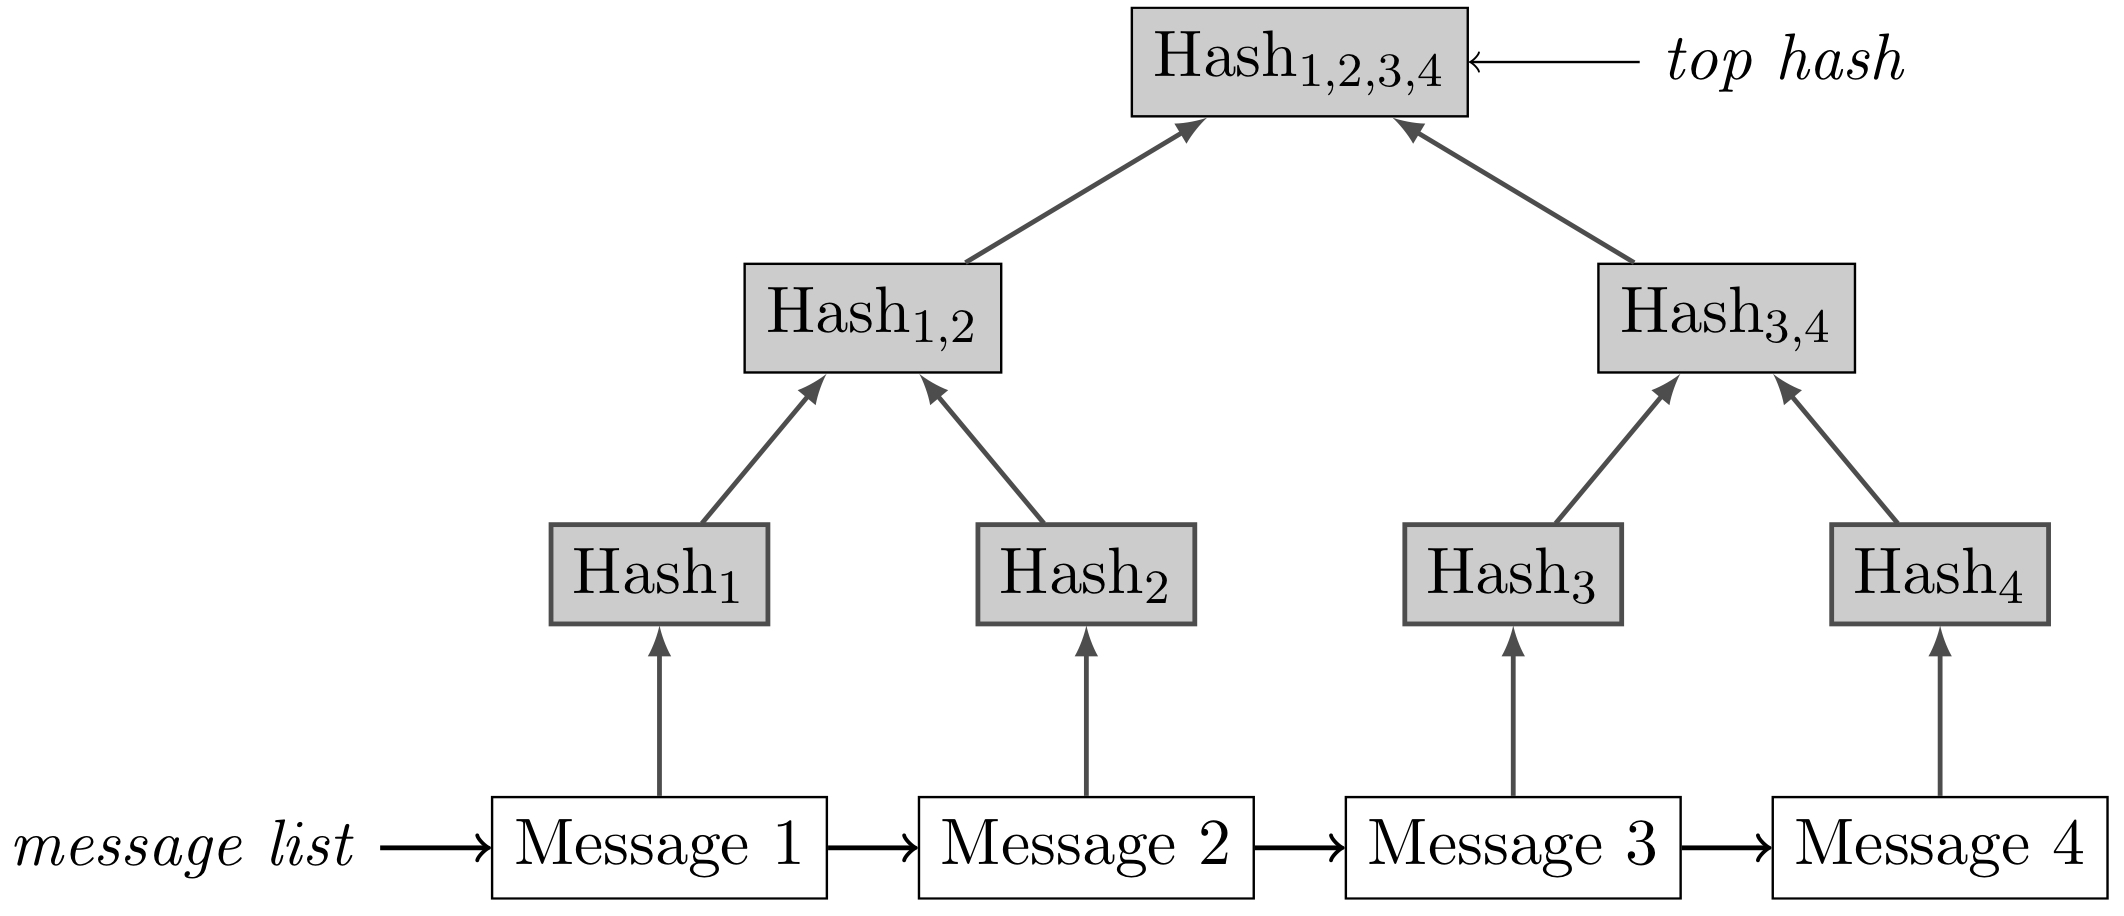
\includegraphics[width=0.85\linewidth]{images/AdvancedDataManagment/distributed_databases/hash_tree.jpeg}
        \caption{A hash tree for four messages}
    \end{figure}
Now, with a hash tree, message list comparison is improved:
\begin{itemize}
    \item When the two top hashes are identical, the two message lists are identical
    \item If the top hashes differ, we go the the next level of the tree and compare the hash values there identical
    \item Whenever we encounter an inner node that has identical hash values in the two hash trees under comparison, then we know that the messages below this inner node are identical
    \item As long as hash values differ for an inner node, we have to go one level deeper and compare the hash values of the child nodes
    \item When we reach a leaf node with different hash values, we have identified a message on which the two message lists differ
\end{itemize}
\newpage
In order to avoid unnecessary hash comparisons, we have to ensure identical root hashes for identical message list. And could be done by:
\begin{itemize}
    \item Let the two servers agree on a sorting order, sort all messages according to this order and then compute the hash tree just before the comparison
    \item Or make each server precompute hash trees for any possible sorting order of the messages. And for comparison the servers then just have to find those two trees with the same sorting order
\end{itemize}